\documentclass[journal,12pt,twocolumn]{IEEEtran}

\usepackage{setspace}
\usepackage{gensymb}

\singlespacing


\usepackage[cmex10]{amsmath}

\usepackage{amsthm}

\usepackage{mathrsfs}
\usepackage{txfonts}
\usepackage{stfloats}
\usepackage{bm}
\usepackage{cite}
\usepackage{cases}
\usepackage{subfig}

\usepackage{longtable}
\usepackage{multirow}

\usepackage{enumitem}
\usepackage{mathtools}
\usepackage{steinmetz}
\usepackage{tikz}
\usepackage{circuitikz}
\usepackage{verbatim}
\usepackage{tfrupee}
\usepackage[breaklinks=true]{hyperref}
\usepackage{graphicx}
\usepackage{tkz-euclide}
\usepackage{float}

\usetikzlibrary{calc,math}
\usepackage{listings}
\usepackage{color} %%
\usepackage{array} %%
\usepackage{longtable} %%
\usepackage{calc} %%
\usepackage{multirow} %%
\usepackage{hhline} %%
\usepackage{ifthen} %%
\usepackage{lscape}
\usepackage{multicol}
\usepackage{chngcntr}

\DeclareMathOperator*{\Res}{Res}

\renewcommand\thesection{\arabic{section}}
\renewcommand\thesubsection{\thesection.\arabic{subsection}}
\renewcommand\thesubsubsection{\thesubsection.\arabic{subsubsection}}

\renewcommand\thesectiondis{\arabic{section}}
\renewcommand\thesubsectiondis{\thesectiondis.\arabic{subsection}}
\renewcommand\thesubsubsectiondis{\thesubsectiondis.\arabic{subsubsection}}


\hyphenation{op-tical net-works semi-conduc-tor}
\def\inputGnumericTable{} %%

\lstset{
%language=C,
frame=single,
breaklines=true,
columns=fullflexible
}
\begin{document}


\newtheorem{theorem}{Theorem}[section]
\newtheorem{problem}{Problem}
\newtheorem{proposition}{Proposition}[section]
\newtheorem{lemma}{Lemma}[section]
\newtheorem{corollary}[theorem]{Corollary}
\newtheorem{example}{Example}[section]
\newtheorem{definition}[problem]{Definition}

\newcommand{\BEQA}{\begin{eqnarray}}
\newcommand{\EEQA}{\end{eqnarray}}
\newcommand{\define}{\stackrel{\triangle}{=}}
\bibliographystyle{IEEEtran}
\providecommand{\mbf}{\mathbf}
\providecommand{\pr}[1]{\ensuremath{\Pr\left(#1\right)}}
\providecommand{\qfunc}[1]{\ensuremath{Q\left(#1\right)}}
\providecommand{\sbrak}[1]{\ensuremath{{}\left[#1\right]}}
\providecommand{\lsbrak}[1]{\ensuremath{{}\left[#1\right.}}
\providecommand{\rsbrak}[1]{\ensuremath{{}\left.#1\right]}}
\providecommand{\brak}[1]{\ensuremath{\left(#1\right)}}
\providecommand{\lbrak}[1]{\ensuremath{\left(#1\right.}}
\providecommand{\rbrak}[1]{\ensuremath{\left.#1\right)}}
\providecommand{\cbrak}[1]{\ensuremath{\left\{#1\right\}}}
\providecommand{\lcbrak}[1]{\ensuremath{\left\{#1\right.}}
\providecommand{\rcbrak}[1]{\ensuremath{\left.#1\right\}}}
\theoremstyle{remark}
\newtheorem{rem}{Remark}
\newcommand{\sgn}{\mathop{\mathrm{sgn}}}
\providecommand{\abs}[1]{\left\vert#1\right\vert}
\providecommand{\res}[1]{\Res\displaylimits_{#1}}
\providecommand{\norm}[1]{\left\lVert#1\right\rVert}
%\providecommand{\norm}[1]{\lVert#1\rVert}
\providecommand{\mtx}[1]{\mathbf{#1}}
\providecommand{\mean}[1]{E\left[ #1 \right]}
\providecommand{\fourier}{\overset{\mathcal{F}}{ \rightleftharpoons}}
%\providecommand{\hilbert}{\overset{\mathcal{H}}{ \rightleftharpoons}}
\providecommand{\system}{\overset{\mathcal{H}}{ \longleftrightarrow}}
%\newcommand{\solution}[2]{\textbf{Solution:}{#1}}
\newcommand{\solution}{\noindent \textbf{Solution: }}
\newcommand{\cosec}{\,\text{cosec}\,}
\providecommand{\dec}[2]{\ensuremath{\overset{#1}{\underset{#2}{\gtrless}}}}
\newcommand{\myvec}[1]{\ensuremath{\begin{pmatrix}#1\end{pmatrix}}}
\newcommand{\mydet}[1]{\ensuremath{\begin{vmatrix}#1\end{vmatrix}}}
\numberwithin{equation}{subsection}
\makeatletter
\@addtoreset{figure}{problem}
\makeatother
\let\StandardTheFigure\thefigure
\let\vec\mathbf
\renewcommand{\thefigure}{\theproblem}
\def\putbox#1#2#3{\makebox[0in][l]{\makebox[#1][l]{}\raisebox{\baselineskip}[0in][0in]{\raisebox{#2}[0in][0in]{#3}}}}
\def\rightbox#1{\makebox[0in][r]{#1}}
\def\centbox#1{\makebox[0in]{#1}}
\def\topbox#1{\raisebox{-\baselineskip}[0in][0in]{#1}}
\def\midbox#1{\raisebox{-0.5\baselineskip}[0in][0in]{#1}}
\vspace{3cm}
\title{Assignment No.4}
\author{Sravani sandya}
\maketitle
\newpage
\bigskip
\renewcommand{\thefigure}{\theenumi}
\renewcommand{\thetable}{\theenumi}
Download all python codes from
\begin{lstlisting}
https://github.com/sravani706/Assignment-4.git
\end{lstlisting}
%
and latex-tikz codes from
%
\begin{lstlisting}
https://github.com/sravani706/Assignment-4.git
\end{lstlisting}
%
Question taken from
\begin{lstlisting}
https://github.com/gadepall/ncert/blob/main/linalg/linear_forms/gvv_ncert_linear_forms.pdf
\end{lstlisting}
\section{Linear Forms Exercise 2.5(b)}
Find out whether the following pair of linear
equations are consistent, or inconsistent.
\begin{align}
    \myvec{2&-3}\vec{x}=8\\
    \myvec{4&-6}\vec{x}=9
\end{align}
\section{Solution}
\begin{align}
    \myvec{2&-3}\vec{x}=8\\
    \myvec{4&-6}\vec{x}=9
\end{align}
The above equations can be expressed as the matrix equation
\begin{align}
     \myvec{2&-3\\4&-6}\vec{x}=\myvec{8\\9}
\end{align}
The augmented matrix for the above equation
is row reduced as follows:
\begin{align}
     \myvec{2& -3& 8\\
           4 & -6 & 9}
          \xleftrightarrow{R_1 \leftarrow{R_1}+3}
    \myvec{5& 0 & 11\\
        4&-6&9}\\
        \xleftrightarrow{R_1\leftarrow\frac{R_1}{5}}
    \myvec{1& 0 &\frac{11}{5}\\4&-6&9}\\
    \xleftrightarrow{R_2\leftarrow{R_2}-4}
    \myvec{1& 0 &\frac{11}{5}\\0&-10& 5}\\
    \xleftrightarrow{R_2\leftarrow \frac{R_2}{10}}
    \myvec{1&0&\frac{11}{5}\\0&-1&\frac{5}{10}}\\
    \xleftrightarrow{R_2 \leftarrow{R_1-R_2}}
    \myvec{1 & 0 & \frac{11}{5}\\ 1 & 1& \frac{17}{10}}\\
    \xleftrightarrow{R_2 \leftarrow{R_2-1}}
    \myvec{1 & 0 & \frac{11}{5} \\ 0 & 0 &\frac{7}{10}}
\end{align}
 So by reduction of the ($2\times3$) matrix
 \begin{align}
     \myvec{2&-3&8\\4&-6&9}
 \end{align}
 Rank of augmented matrix is 2. 
   \begin{align}
       \myvec{2&-3\\4&-6}
   \end{align} 
 The rank of the above matrix is 1.\\
 Hence the rank of two matrix are not equal\\
   $\therefore$ lines are Inconsistent.
  \numberwithin{figure}{section}
\begin{figure}[H]
    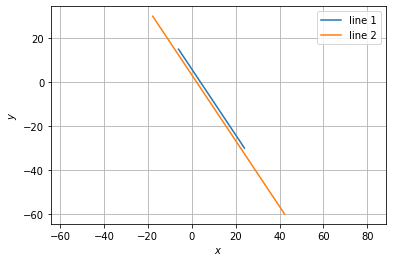
\includegraphics[width= \columnwidth]{download4.png}
    \caption{Graphical solution}
    \label{Fig:Graphical Solution}
\end{figure}
$\therefore$ This figure verifies that two lines are  not intersecting at one point.
\end{document}
